\documentclass[letter,12pt]{scrartcl}
\usepackage{amsmath,amssymb}
\usepackage[latin1]{inputenc}
\usepackage{standalone}
\usepackage{tikz,pgf,pgfplots}
\usetikzlibrary{decorations.pathmorphing}

\usepackage[margin=20mm]{geometry}
\newenvironment{exercise}[1][Uppgift]{\begin{trivlist} \item[\hskip
    \labelsep {\stepcounter{exerctr}\bfseries #1
      \arabic{exerctr}}]}{\end{trivlist}\vspace{10mm}}

\newcounter{exerctr}
\newcounter{abcctr}[exerctr]

\newcommand{\abc}{\noindent\vspace{1mm}\\ {\bf
    \stepcounter{abcctr}(\alph{abcctr})\ }}
\newcommand{\bbm}{\begin{bmatrix}}
\newcommand{\ebm}{\end{bmatrix}}
\newcommand{\point}[1]{\hfill {\bf (#1p)}\\ \vspace{-5mm}}
\newcommand{\ctrb}{\EuScript{S}}
\newcommand{\Lap}{\mathcal{L}}
\newcommand{\obsv}{\EuScript{O}}
\newcommand{\realdel}[1]{\text{Re}\left\{#1\right\}}
\newcommand{\imagdel}{\text{Im}}
\newcommand{\bC}{\mathbb{C}}
\newcommand{\bR}{\mathbb{R}}
\newcommand{\bmpv}{\begin{minipage}[t]}
\newcommand{\bmps}{\begin{minipage}[t]{45mm}}
\newcommand{\bmpm}{\begin{minipage}[t]{90mm}}
\newcommand{\bmpl}{\begin{minipage}[t]{\textwidth}}
\newcommand{\emp}{\end{minipage}}
\newcommand*{\zethree}{\big(z - \mexp{-3h}\big)}
\newcommand*{\mexp}[1]{\ensuremath{\mathrm{e}^{#1}}}

\newcommand*\circled[1]{\tikz[baseline=(char.base)]{
            \node[shape=circle,draw,inner sep=2pt] (char) {#1};}}

\tikzset{
   ragged border/.style={ decoration={random steps, segment length=1mm, amplitude=0.5mm},
           decorate,
   }
}


\title{Computerized control partial exam 1 (15\%)}
\author{Kjartan Halvorsen}

\begin{document}

\maketitle


\begin{description}
\item[Time] February 10 17:30
\item[Place] 5105
\item[Permitted aids] The single colored page with your own notes, table of Laplace transforms, calculator
\end{description}

All answers should be readable and well motivated (if nothing else is written). Solutions/motivations should be written on the provided spaces in this exam. Use the last page if more space is needed.

\begin{center}
{\Large Good luck!} \\
\end{center}

\begin{tabular}{|l|l|}
\hline
\multicolumn{2}{|l|}{\bmpl
Matricula and name
\vspace*{18mm}
\emp}\\
\hline

\end{tabular}

\clearpage

%-----------------------------------------------------------------
\subsection*{The system}

Consider the water tank illustrated in figure \ref{fig:tank_ill}.  After linearization and with certain values for the parameters $A$, $a$, and $h_0$, the system leads to the model shown in figure \ref{fig:tank}. Note that the variables are defined as deviations from some nominal values, i.e.~deviations from an operating point. There is a valve controlling the flow of water into the tank, and $u(t)$ is the control signal to the valve. When the pressure in the water pipe is at the normal level, the valve reacts to the control signal with the (change in) flow $\bar{w}(t)$. Varying water pressure leads to variations in the actual flow, and this is modelled as an additive disturbance $v(t)$, so the actual change in flow is $w(t) = \bar{w}(t) + v(t)$. 
\begin{figure}[h]
  \begin{center}
    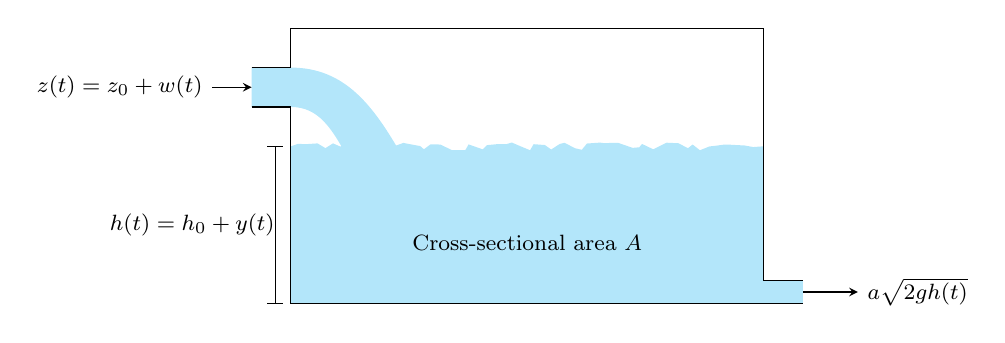
\begin{tikzpicture}
      \fill[cyan!30]
      decorate[ragged border]{
        (0,2) -- (6,2)
      }
      -- (6,0.3) -- (6.5,0.3) -- (6.5,0.0) -- (6,0.0) --(6,0) -- (0,0) -- cycle;
      \fill[cyan!30] (-0.5,2.5) -- (0,2.5) to[in=120,out=0](0.7,1.9)-- (1.4,1.9)
      to[out=120,in=0] (0,3) -- (-0.5,3) -- cycle;
      \draw (-0.5,2.5) -- (0,2.5) -- (0,0) -- (6,0) -- (6,0.0) -- (6.5,0.0);
      \draw (-0.5,3) -- (0,3) -- (0,3.5) -- (6,3.5) -- (6,0.3) -- (6.5,0.3);
      \draw[|-|] (-0.2,0) --
      node[fill=white,font=\footnotesize,inner ysep=2pt,inner
      xsep=0, anchor=east]{$h(t) = h_0 + y(t)$}(-0.2,2);
      \draw[stealth-] (-0.5,2.75) -- (-1,2.75)
      node[anchor=east,font=\footnotesize,align=right]{$z(t) = z_0 + w(t)$};
      \draw[-stealth] (6.5,0.15) -- (7.2,0.15)
      node[anchor=west,font=\footnotesize]{$a\sqrt{2gh(t)}$};
      \node[anchor=north,font=\footnotesize] at (3,3) {};
      \node[anchor=north,font=\footnotesize] at (3,2) {};
      \node[anchor=north,font=\footnotesize] at (3,1) {Cross-sectional area $A$};
    \end{tikzpicture}%
    \caption{Tank with hole in the bottom.}
    \label{fig:tank_ill}
  \end{center}
\end{figure}


\begin{figure}[h]
  \begin{center}
    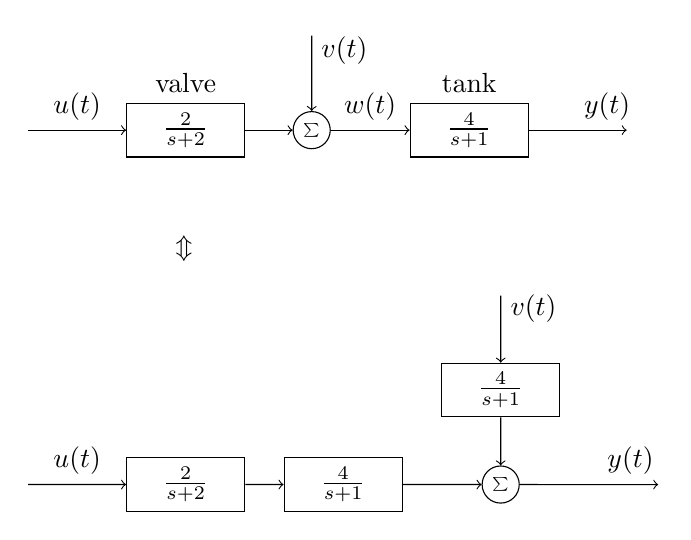
\begin{tikzpicture}[scale = 0.8, node distance=20mm, block/.style={rectangle, draw, minimum width=15mm}, sumnode/.style={circle, draw, inner sep=2pt}]
      
      %\node[coordinate] (refinput) {};
      %\node[sumnode, right of=refinput, node distance=20mm] (sumerr) {\tiny $\sum$};
      %\node[block, right of=sumerr] (controller) {$K$};
      %\node[above of=controller, node distance=6mm] {controller};
      
      %\node[block, right of=controller, node distance=24mm] (valve) {$\frac{2}{s+2}$};
      \node[block,] (valve) {$\frac{2}{s+2}$};
      \node[above of=valve, node distance=6mm] {valve};
      \node[sumnode, right of=valve, node distance=16mm] (sum) {\tiny $\sum$};
      \node[block, right of=sum, node distance=20mm] (tank) {$\frac{4}{s+1}$};
      \node[above of=tank, node distance=6mm] {tank};
      \node[coordinate, right of=tank, node distance=20mm] (output) {};
      \node[coordinate, above of=sum, node distance=12mm] (disturbance) {};
      \node[coordinate, left of=valve, node distance=20mm] (input) {};

      %\draw[->] (refinput) -- node[above, pos=0.3] {$y_{ref}(t)=0$} (sumerr);
      %\draw[->] (sumerr) -- node[above] {$e(t)$} (controller);
      %\draw[->] (controller) -- node[above] {$u(t)$} (valve);
      \draw[->] (input) -- node[above] {$u(t)$} (valve);
      \draw[->] (valve) -- node[above] {} (sum);
      \draw[->] (sum) -- node[above] {$w(t)$} (tank);
      \draw[->] (tank) -- node[coordinate] (measure) {} node[above, pos=0.8] {$y(t)$} (output);
      \draw[->] (disturbance) -- node[right, pos=0.2] {$v(t)$} (sum);
      %\draw[->] (measure) -- ++(0,-14mm) -| node[right, pos=0.95] {$-$} (sumerr);


      \node[below of= valve, node distance=15mm, rotate=90] (equiv) {$\Leftrightarrow$};

      \node[block, below of=equiv, node distance=30mm] (valve) {$\frac{2}{s+2}$};
      \node[block, right of=valve, node distance=20mm] (tank) {$\frac{4}{s+1}$};
      \node[sumnode, right of=tank, node distance=20mm] (sum) {\tiny $\sum$};
      \node[coordinate, right of=sum, node distance=20mm] (output) {};
      \node[block, above of=sum, node distance=12mm] (tank2) {$\frac{4}{s+1}$};
      \node[coordinate, above of=tank2, node distance=12mm] (disturbance) {};
      \node[coordinate, left of=valve, node distance=20mm] (input) {};

      %\draw[->] (refinput) -- node[above, pos=0.3] {$y_{ref}(t)=0$} (sumerr);
      %\draw[->] (sumerr) -- node[above] {$e(t)$} (controller);
      %\draw[->] (controller) -- node[above] {$u(t)$} (valve);
      \draw[->] (input) -- node[above] {$u(t)$} (valve);
      \draw[->] (valve) -- node[above] {} (tank);
      \draw[->] (tank) -- node[above] {} (sum);
      \draw[->] (sum) -- node[coordinate] (measure) {} node[above, pos=0.8] {$y(t)$} (output);
      \draw[->] (disturbance) -- node[right, pos=0.2] {$v(t)$} (tank2);
      \draw[->] (tank2) -- node[above] {} (sum);
      %\draw[->] (measure) -- ++(0,-14mm) -| node[right, pos=0.95] {$-$} (sumerr);

    \end{tikzpicture}
    \caption{Tank model with valve.}
    \label{fig:tank}
  \end{center}
\end{figure}
\clearpage
\subsection*{Problem 1 (50p)}

Discretizing the system using step-invariant (zero-order-hold) sampling with sampling interval $h$ gives the discrete-time system shown in figure \ref{fig:block}. \textbf{Show that the two pulse-transfer functions \(H_1(z)\) and \(H_2(z)\) are given by}
   \begin{align*}
   H_1(z) &= \frac{4(z-\mexp{-h})(z-\mexp{-2h}) - 8(z-1)(z-\mexp{-2h}) + 4(z-1)(z-\mexp{-h})}{(z-\mexp{-h})(z-\mexp{-2h})}\\
        &= \frac{ \big( 4 - 8\mexp{-h} +4\mexp{-2h}\big) z + 4\mexp{-h}(\mexp{-2h} +1 ) -8\mexp{-2h}}{(z-\mexp{-h})(z-\mexp{-2h})}\\
   H_2(z) &= \frac{4(1-\mexp{-h})}{z-\mexp{-h}}.
   \end{align*}
   
\begin{figure}[h]
  \begin{center}
    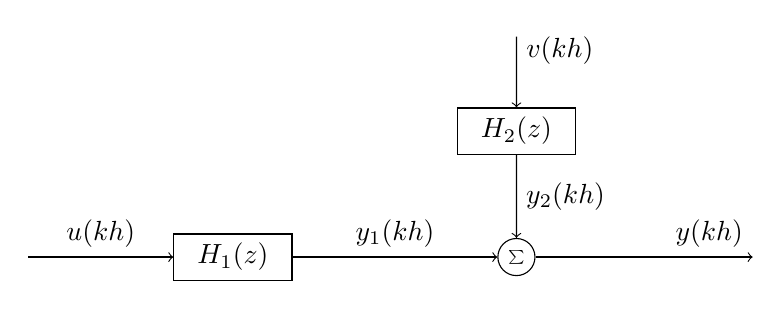
\begin{tikzpicture}[scale = 0.6, node distance=20mm, block/.style={rectangle, draw, minimum width=15mm}, sumnode/.style={circle, draw, inner sep=2pt}]

      \node[block] (valve) {$H_1(z)$};
      \node[sumnode, right of=valve, node distance=36mm] (sum) {\tiny $\sum$};
      \node[coordinate, right of=sum, node distance=30mm] (output) {};
      \node[block, above of=sum, node distance=16mm] (tank2) {$H_2(z)$};
      \node[coordinate, above of=tank2, node distance=12mm] (disturbance) {};
      \node[coordinate, left of=valve, node distance=26mm] (input) {};

      \draw[->] (input) -- node[above] {$u(kh)$} (valve);
      \draw[->] (valve) -- node[above] {$y_1(kh)$} (sum);
      \draw[->] (sum) -- node[coordinate] (measure) {} node[above, pos=0.8] {$y(kh)$} (output);
      \draw[->] (disturbance) -- node[right, pos=0.2] {$v(kh)$} (tank2);
      \draw[->] (tank2) -- node[right] {$y_2(kh)$} (sum);
      %\draw[->] (measure) -- ++(0,-14mm) -| node[right, pos=0.95] {$-$} (sumerr);

    \end{tikzpicture}
    \caption{Discrete-time model of tank with valve.}
    \label{fig:block}
  \end{center}
\end{figure}

\noindent
\fbox{
\bmpl
{\bf Derivation:}\\
\vspace*{120mm}
\emp}

\clearpage
\subsection*{Problem 2 (20p)}
Assume that the sampling period is $h=0.2$. In figure \ref{fig:complex-plane} draw the poles (crosses) and zero (circle) for both the continuous-time plant model $G_1(s)$ and the  discretized pulse-transfer function $H_1(z)$ you determined in Problem 1.
   \begin{figure}[h]
   \begin{center}
   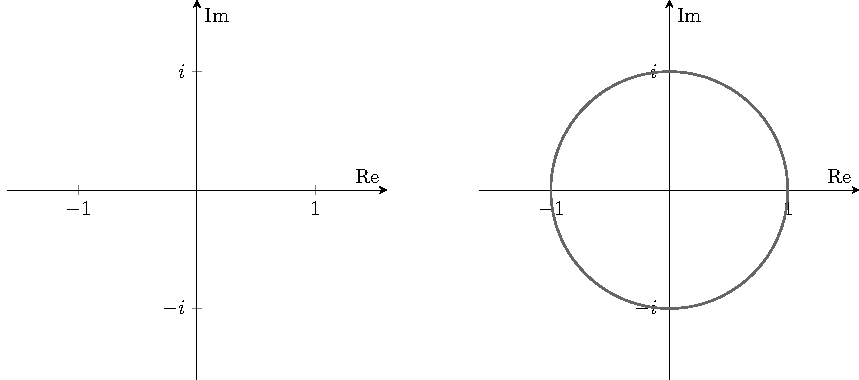
\includegraphics[]{complex-plane}
   \caption{Problem 2: Plot the poles of the continuous-time system (on the left) and the poles and zero of the discrete-time system (on the right). Indicate (with arrows and/or colors) corresponding pairs of continuous-time and discrete-time poles.}
   \label{fig:complex-plane}
   \end{center}
   \end{figure}

\noindent
\fbox{
\bmpl
{\bf Calculations:}\\
\vspace*{100mm}
\emp}

\clearpage

\subsection*{Problem 3 (30p)}
The tank model is controlled using the feedback controller \(F(z) = K \frac{1.1z - 0.9}{z-1}\). See figure \ref{fig:feedback}. 
\begin{figure}
\begin{center}
    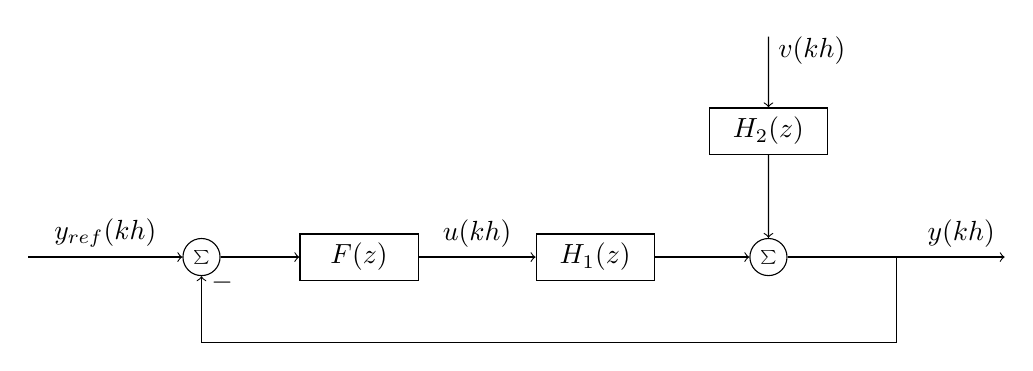
\begin{tikzpicture}[scale = 0.6, node distance=20mm, block/.style={rectangle, draw, minimum width=15mm}, sumnode/.style={circle, draw, inner sep=2pt}]

      \node[block] (valve) {$H_1(z)$};
      \node[sumnode, right of=valve, node distance=22mm] (sum) {\tiny $\sum$};
      \node[coordinate, right of=sum, node distance=30mm] (output) {};
      \node[block, above of=sum, node distance=16mm] (tank2) {$H_2(z)$};
      \node[coordinate, above of=tank2, node distance=12mm] (disturbance) {};
      %\node[coordinate, left of=valve, node distance=26mm] (input) {};
      \node[block, left of=valve, node distance=30mm] (controller) {$F(z)$};
      \node[sumnode, left of=controller, node distance=20mm] (refsum) {\tiny $\sum$};
      \node[coordinate, left of=refsum, node distance=22mm] (refinput) {};
      
      \draw[->] (refinput) -- node[above] {$y_{ref}(kh)$} (refsum);
      \draw[->] (refsum) -- node[above] {} (controller);
      \draw[->] (controller) -- node[above] {$u(kh)$} (valve);
      \draw[->] (valve) -- node[above] {} (sum);
      \draw[->] (sum) -- node[coordinate] (measure) {} node[above, pos=0.8] {$y(kh)$} (output);
      \draw[->] (disturbance) -- node[right, pos=0.2] {$v(kh)$} (tank2);
      \draw[->] (tank2) -- node[right] {} (sum);
      \draw[->] (measure) -- ++(0,-18mm) -| node[right, pos=0.95] {$-$} (refsum);
     
     \end{tikzpicture}
     \caption{Feedback control from the error signal.}
     \label{fig:feedback}
   \end{center}
 \end{figure}
 

Figure~\ref{fig:rlocus} shows the root locus for the closed-loop poles with respect to the gain $K$. In figure~\ref{fig:step}, four different closed-loop responses to a step disturbance in the water pressure are shown. The different responses are for four different values of $K$. Identify (and circle) the corresponding step plot for each value of $K$ in the table below. \textbf{Motivate your choice!}

\begin{center}
\begin{tabular}{cl}
\(K\) & Step plot\\\hline
0.1 & A\hspace*{2mm} B\hspace*{2mm} C\hspace*{2mm} D\\
0.8 & A\hspace*{2mm}  B\hspace*{2mm}  C\hspace*{2mm} D\\
2.0 & A\hspace*{2mm} B\hspace*{2mm}  C\hspace*{2mm} D\\
4.0 & A\hspace*{2mm} B\hspace*{2mm}  C\hspace*{2mm} D\\ \hline
\end{tabular}
\end{center}

\begin{figure}[h]
\begin{center}
\begin{tikzpicture}
    \node[anchor=south west,inner sep=0] at (0,0) {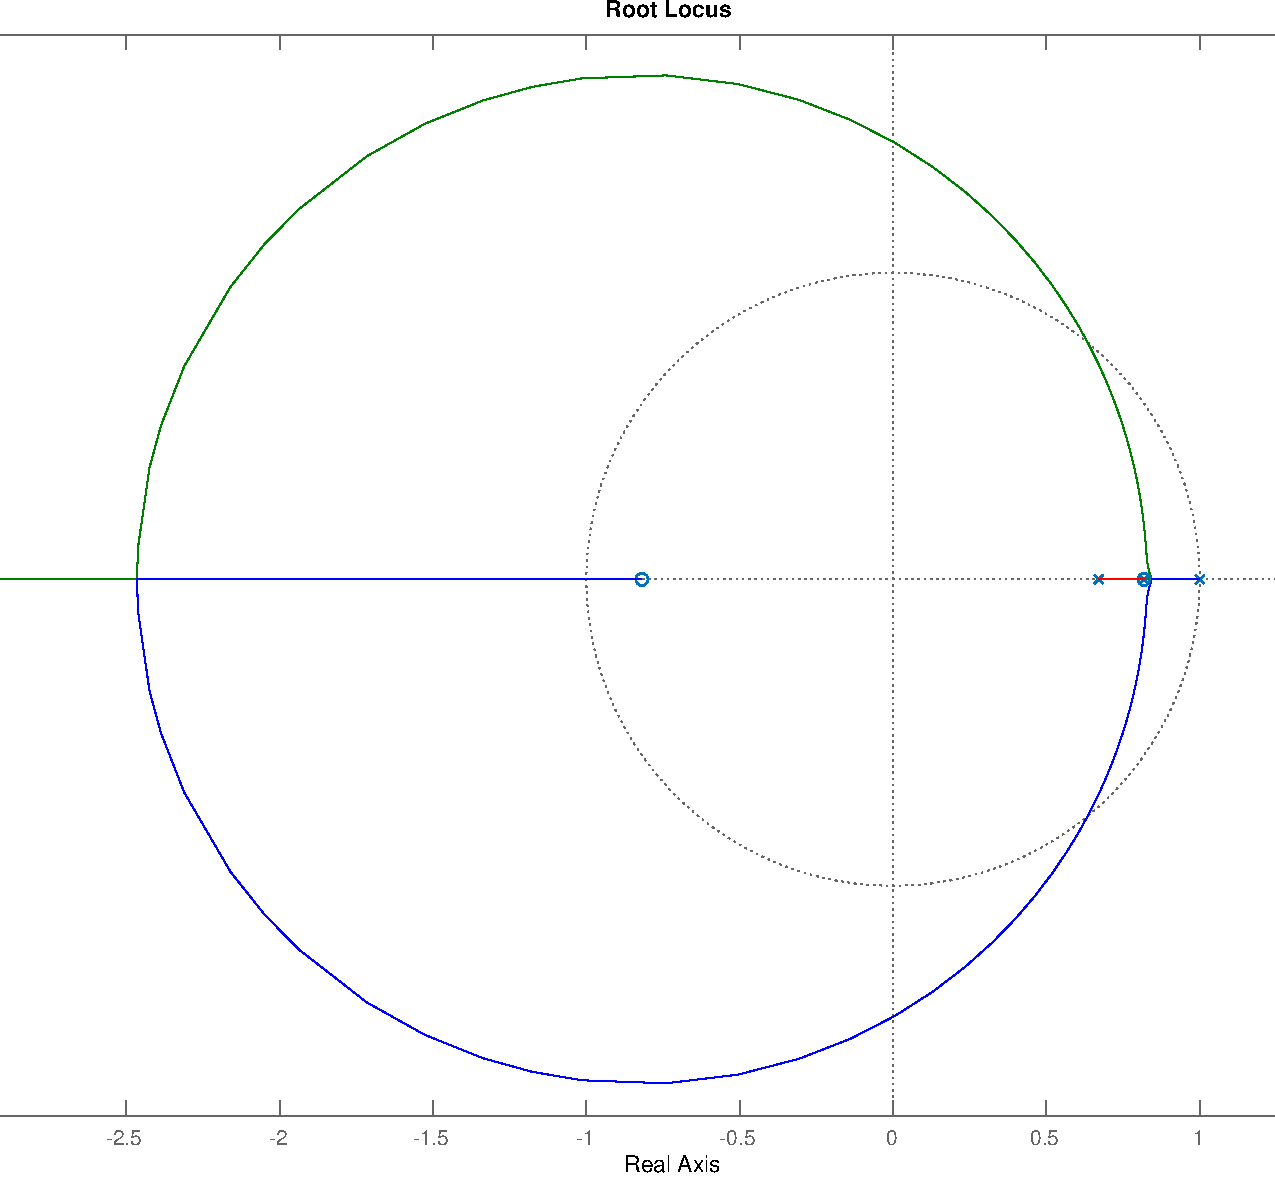
\includegraphics[width=0.6\linewidth]{p3_rlocus-crop}};
    \node[coordinate, pin={[pin distance=20mm] 10:{$K=0.1$}}] at (9.17,4.9) {};
    \node[coordinate, pin={[pin distance=20mm] 60:{$K=2.2$}}] at (8.75,6.6) {};
\end{tikzpicture} 

\caption{Root locus wrt the gain $K$.}
\label{fig:rlocus}
\end{center}
\end{figure}

\begin{figure}[t]
\begin{center}
\begin{tabular}{cc}
A & B\\
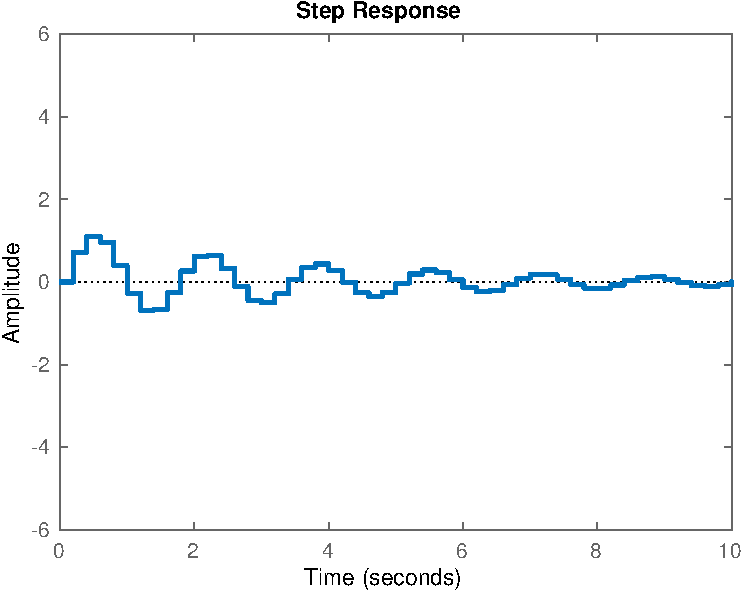
\includegraphics[width=0.4\linewidth]{step-plot-3-crop}
&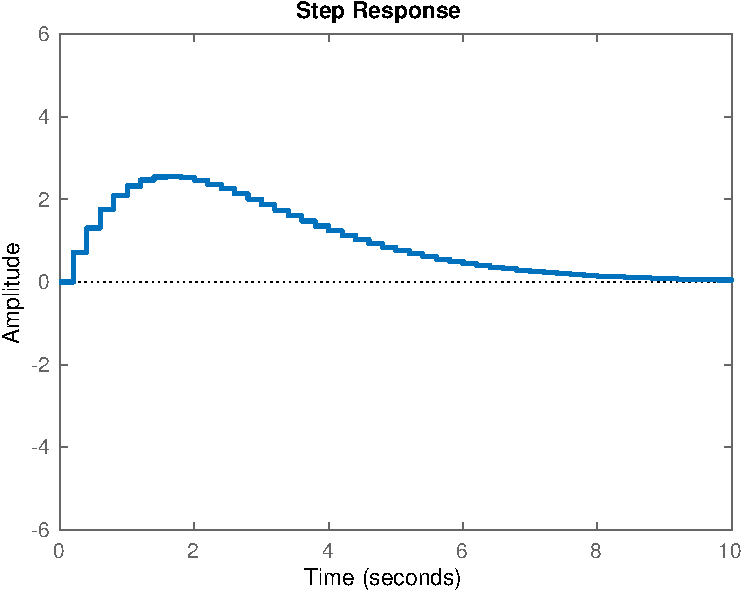
\includegraphics[width=0.4\linewidth]{step-plot-1-crop}\\
C & D\\
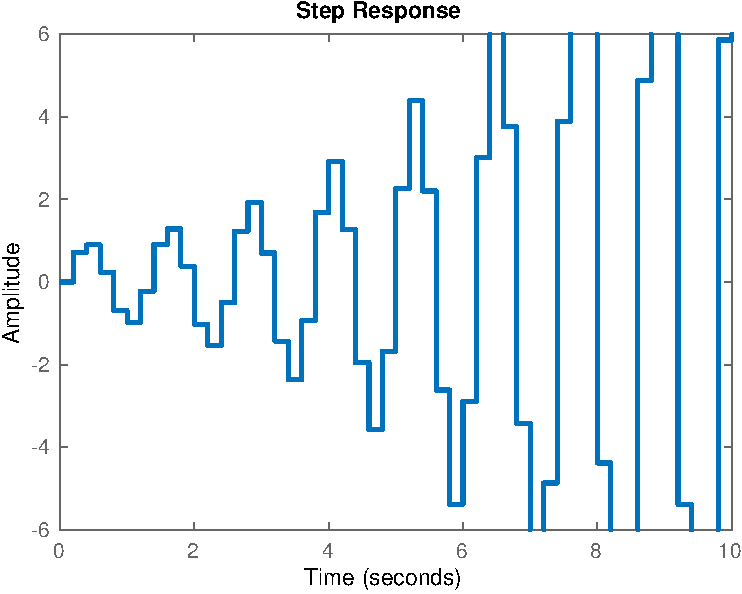
\includegraphics[width=0.4\linewidth]{step-plot-5-crop}
&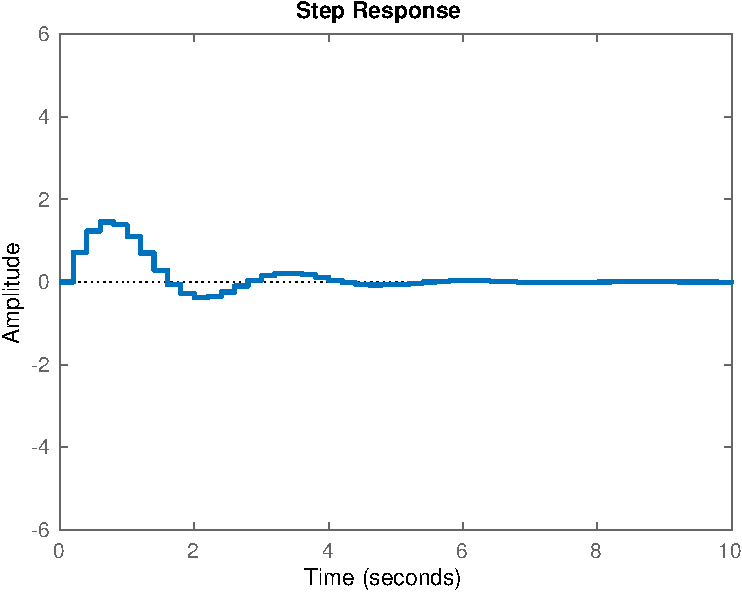
\includegraphics[width=0.4\linewidth]{step-plot-2-crop}

\end{tabular}
\caption{Step responses for different values of $K$.}
\label{fig:step}
\end{center}
\end{figure}

\noindent
\fbox{
\bmpl
{\bf Motivation:}\\
\vspace*{80mm}
\emp}


\clearpage

\noindent
{\bf If necessary,} you can continue your solutions on this page. Mark clearly which problem the solution corresponds to.


%\end{document}

%*****************************************************************
%*****************************************************************
\newpage
\setcounter{page}{1}

\section*{Solutions}
\subsection*{Problem 1}
   There are two continous-time systems to discretize \(G_1(s) = \frac{8}{(s+1)(s+2)}\) and \(G_2(s) = \frac{4}{s+1}\). First calculate the step-response of the system \(G_1(s)\)
   \[Y_1(s) = G_1(s)\frac{1}{s} = \frac{8}{s(s+1)(s-1)} = \frac{4}{s} - \frac{8}{s+1} + \frac{4}{s+2}.\]
   The inverse Laplace-transform gives
   \[ y_1(t) = \left(4 - 8\mexp{-t} +4\mexp{-2t}\right)u_H(t),\]
   where $u_H(t)$ is the Heaviside step function. Sampling $y(t)$ gives
   \[ y_1(kh) = \left(4 - 8\mexp{-kh} +4\mexp{-2kh}\right)u_H(kh),\]
   which has the Z-transform
   \[Y_1(z) = \frac{4z}{z-1} - \frac{8z}{z - \mexp{-h}} + \frac{4z}{z - \mexp{-2h}}.\]
   Dividing the z-transform of the system response to that of the input (the step) gives
   \begin{align*}
   H_1(z) &= \frac{Y_1(z)}{U(z)} = \frac{z-1}{z}Y_1(z) = 4 - \frac{8(z-1)}{z-\mexp{-h}} + \frac{4(z-1)}{z-\mexp{-2h}}\\
        &= \frac{4(z-\mexp{-h})(z-\mexp{-2h}) - 8(z-1)(z-\mexp{-2h}) + 4(z-1)(z-\mexp{-h})}{(z-\mexp{-h})(z-\mexp{-2h})}\\
        &= \frac{4z^2 - 4(\mexp{-h} + \mexp{-2h})z + 4\mexp{-h}\mexp{-2h} - 8z^2 +8(1+\mexp{-2h})z - 8\mexp{-2h} + 4z^2 - 4(1+\mexp{-h})z + 4\mexp{-h}}{(z-\mexp{-h})(z-\mexp{-2h})}\\
        &= \frac{ \big( - 4\mexp{-h} -4\mexp{-2h} +8 + 8\mexp{-2h} -4 -4\mexp{-h}\big) z + 4\mexp{-h}\mexp{-2h} -8\mexp{-2h} +4\mexp{-h}}{(z-\mexp{-h})(z-\mexp{-2h})}\\
        &= \frac{ \big( 4 - 8\mexp{-h} +4\mexp{-2h}\big) z + 4\mexp{-h}(\mexp{-2h} +1 ) -8\mexp{-2h}}{(z-\mexp{-h})(z-\mexp{-2h})}
   \end{align*}

   The same procedure for the system \(G_2(s)\) gives 
   \[Y_2(s) = G_2(s)\frac{1}{s} = \frac{4}{s(s+1)} = \frac{4}{s} - \frac{4}{s+1}.\] Inverse Laplace gives
   \[y_2(t) = (4 - 4\mexp{-t})u_H(t), \] which sampled is 
   \[y_2(kh) = (4 - 4\mexp{-kh})u_H(kh).\] The z-transform gives
   \[Y_2(z) = \frac{4z}{z-1} - \frac{4z}{z-\mexp{-h}}.\] Dividing with the z-transform of the step input gives 
   \begin{align*}
   H_2(z) &= \frac{Y_2(z)}{U(z)} = \frac{z-1}{z}Y_2(z) = 4 - \frac{4(z-1)}{z-\mexp{-h}}\\
          &= \frac{4(z-\mexp{-h}) - 4(z-1)}{z-\mexp{-h}} = \frac{4(1-\mexp{-h})}{z-\mexp{-h}}.
   \end{align*}
   

\subsection*{Problem 2}
The discrete-time poles are in $z=\mexp{-h}=\mexp{-0.2}$ and $z=\mexp{-2h}=\mexp{-0.4}$. The zero is  in 
\[ z = - \frac{4\mexp{-h}(\mexp{-2h} +1 ) -8\mexp{-2h}}{ 4 - 8\mexp{-h} +4\mexp{-2h}} \approx -0.82\]
\begin{center}
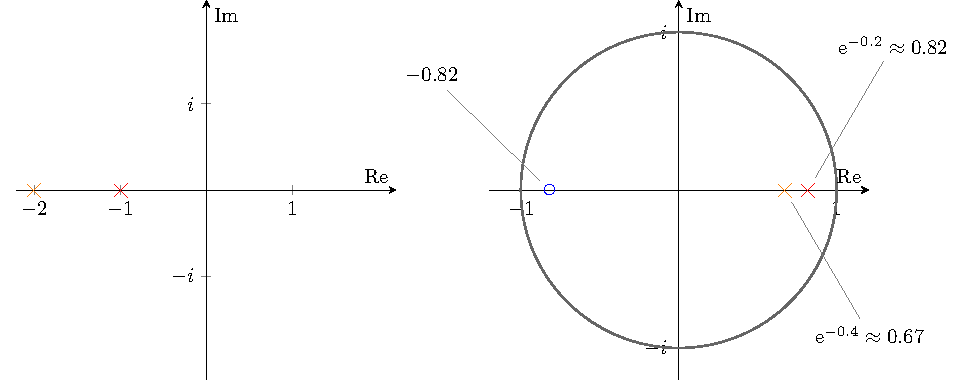
\includegraphics[width=0.8\linewidth]{complex-plane-facit-vt17}
\end{center}
 
\subsection*{Problem 3}
From the root locus we see that if the gain is $K>2.2$, then the closed-loop system will have two complex-conjugated poles outside the unit circle, and the system will be unstable. So the gain $K=4$ should give an unstable response. This is seen in the response C. As the gain increases from 0.1 we should see responses that are increasingly faster and with more pronounced and faster oscillations. Hence response B corresponds to the most damped and slowest response, response D is faster and with some damping, and finally response A has little damping and quite fast oscillations. 

\begin{center}
\begin{tabular}{cl}
\(K\) & Step plot\\\hline
0.1 & A\hspace*{2mm} \circled{B}\hspace*{2mm} C\hspace*{2mm} D\\
0.8 & A\hspace*{2mm}  B\hspace*{2mm}  C\hspace*{2mm} \circled{D}\\
2.0 & \circled{A}\hspace*{2mm} B\hspace*{2mm}  C\hspace*{2mm} D\\
4.0 & A\hspace*{2mm} B\hspace*{2mm}  \circled{C}\hspace*{2mm} D\\ \hline
\end{tabular}
\end{center}


\end{document}
